\documentclass[12pt,a4paper]{article}
\usepackage[utf8]{inputenc}
\usepackage{amsmath}
\usepackage{amsfonts}
\usepackage{amssymb}
\usepackage{lipsum}
\usepackage{textcomp}

\usepackage{makecell} % linebreak dans une cellule
\usepackage{multicol} % twocols localement
\usepackage{vwcol} % idem mais avec largeur variable
\usepackage{color, colortbl} % colorer les tableaux
\usepackage{enumitem} % utiliser des lettres pour énumérer
\usepackage{wrapfig} % insérer des images dans dutexte
\usepackage{dashundergaps} % transformer du texte en ________
\usepackage{MnSymbol,wasysym} % smileys
\usepackage{minibox} % multiline fbox - \minibox[frame]{}
\usepackage[pscoord]{eso-pic} % floating text box \placetextbox{x}{y}{text}
\usepackage{ifthen}
\usepackage{soul} % teste barré \st

% --- geometry ---
\usepackage{geometry}
\geometry{legalpaper, margin=1cm}
% ---

% --- xcolor ---
\usepackage{xcolor}
\definecolor{lightgray}{gray}{0.9}
% ---

% --- tcolorboxes ---
\usepackage[most]{tcolorbox}
\newtcolorbox{definition}[2][]{%
  attach boxed title to top left
               = {yshift=-8pt},
  colback      = white,
  colframe     = gray,
  fonttitle    = \bfseries,
  colbacktitle = gray,
  title        = #2,#1,
  enhanced,
}
% ---

% --- array ---
\usepackage{array}
\newcolumntype{L}[1]{>{\raggedright\let\newline\\\arraybackslash\hspace{0pt}}m{#1}}
\newcolumntype{C}[1]{>{\centering\let\newline\\\arraybackslash\hspace{0pt}}m{#1}}
\newcolumntype{R}[1]{>{\raggedleft\let\newline\\\arraybackslash\hspace{0pt}}m{#1}}
 % ---


\renewcommand{\baselinestretch}{1.15} % augmenter l'interligne

\dashundergapssetup{
	teacher-gap-format=underline,
	gap-widen
}

\newcommand{\placetextbox}[3]{% \placetextbox{<horizontal pos>}{<vertical pos>}{<stuff>}
  \setbox0=\hbox{#3}% Put <stuff> in a box
  \AddToShipoutPictureFG*{% Add <stuff> to current page foreground
    \put(\LenToUnit{#1\paperwidth},\LenToUnit{#2\paperheight}){\vtop{{\null}\makebox[0pt][c]{#3}}}%
  }%
}%


\author{Paul Clavier}
\title{Chapitre 4 - Comparaison de nombres décimaux - Interrogation} 

\begin{document}

% --- Section & subsection renum ---
\renewcommand\thesection{\Roman{section}}
\renewcommand\thesubsection{\arabic{subsection}}
% ---

% --- Selection manuelle de la version ---
%\def\isprof{true}
% ---

% --- Selection automatique de la version ---
\ifdefined\isprof
	\TeacherModeOn
\fi

% ---

\begin{center}
	\minibox[frame,c]{Chapitre 4 - Comparaison de nombres décimaux \\ Interrogation Écrite}
\end{center}

\placetextbox{0.1}{0.99}{Nom:}
\placetextbox{0.1}{0.96}{Prénom:}

\begin{center}
\begin{tabular}{|l|c|}
\hline \rowcolor{lightgray}
Les nombres décimaux \hspace{8cm} & Maitrise \\ \hline
\thead[l]{1.3: Utiliser et représenter les grands nombres entiers, des fractions simples, les nombres décimaux} &
\\ \hline
\thead[l]{1.3:Utiliser des notions de géométrie plane} &
 \\ \hline
\end{tabular}
\end{center}

\textbf{Exercice 1}: QCM

Dans le tableau ci dessous, entoure la ou les bonne(s) réponse(s)
\begin{center}
\begin{tabular}{|c|c|c|c|c|}
\hline 
\thead{Nomme la figure \\ \includegraphics[scale=0.5]{"img/IE - demidroite-AB".png}}  & [AB] & (AB) & [AB) & (AB] \\ 
\hline 
\thead{Quel est le plus grand nombre? } & 1,74 & 1,699 & 0,99 & 1,73 \\ 
\hline 
\thead{Quelle est la partie entière de 17,89 ?} & 7 & 17 & 89 & 0,89 \\ 
\hline 
\thead{Dans 24,691 combien y a t'il de centièmes?} & 69 & 2 469 & 24 691 & 0,691 \\ 
\hline 
\end{tabular}
\end{center}

\textbf{Exercice 2}: Donne l'abscisse des points suivants\\

\begin{minipage}{0.4\textwidth}
\begin{center}
\begin{tikzpicture}
\draw (0,0) -- (4,0);
\foreach \x in {0,1,...,4} {\draw (\x,0.1cm) -- (\x,-0.1cm) node[below] {$\x\strut$};}
\foreach \x in {0,0.1,...,4} {\draw (\x,0.05cm) -- (\x,-0.05cm);}
\draw (1.3cm,0.25cm) -- (1.3cm,-0.25cm) node[above=0.4cm] {A\strut};
\end{tikzpicture}\\
A(\gap*{1,3})
\end{center}
\end{minipage}
\begin{minipage}{0.4\textwidth}
\begin{center}
\begin{tikzpicture}
\draw (0,0) -- (4,0);
\foreach \x in {0,1} {\draw (\x,0.1cm) -- (\x,-0.1cm) node[below] {$\x\strut$};}
\foreach \x in {2,...,4} {\draw (\x,0.1cm) -- (\x,-0.1cm);}
\foreach \x in {0,0.1,...,4} {\draw (\x,0.05cm) -- (\x,-0.05cm);}
\draw (3.1cm,0.25cm) -- (3.1cm,-0.25cm) node[above=0.4cm] {B\strut};
\end{tikzpicture}\\
B(\gap*{3,1})
\end{center}
\end{minipage}

\begin{minipage}{0.4\textwidth}
\begin{center}
\begin{tikzpicture}
\draw (0,0) -- (4,0);
\foreach \x in {0,1,...,4} {\draw (\x,0.1cm) -- (\x,-0.1cm);}
\draw (3,0.1cm) -- (3,-0.1cm) node[below] {$4$};
\draw (4,0.1cm) -- (4,-0.1cm) node[below] {$5$};
\foreach \x in {0,0.1,...,4} {\draw (\x,0.05cm) -- (\x,-0.05cm);}
\draw (1.4cm,0.25cm) -- (1.4cm,-0.25cm) node[above=0.4cm] {C\strut};
\end{tikzpicture}\\
C(\gap*{2,4})
\end{center}
\end{minipage}
\begin{minipage}{0.4\textwidth}
\begin{center}
\begin{tikzpicture}
\draw (0,0) -- (4,0);
\foreach \x in {0,1,...,4} {\draw (\x,0.1cm) -- (\x,-0.1cm) ;}
\foreach \x in {0,0.2,...,4} {\draw (\x,0.05cm) -- (\x,-0.05cm);}
\draw (2,0.1cm) -- (2,-0.1cm) node[below] {$0,6$};
\draw (4,0.1cm) -- (4,-0.1cm) node[below] {$0,7$};
\draw (0.7cm,0.25cm) -- (0.7cm,-0.25cm) node[above=0.4cm] {D\strut};
\end{tikzpicture}\\
D(\gap*{0,535})
\end{center}
\end{minipage}

\textbf{Exercice 3}: Place les points d'abscisse suivants

\begin{center}
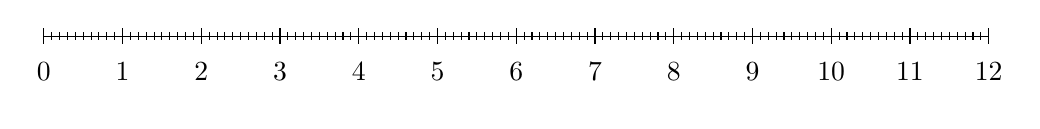
\begin{tikzpicture}
\draw (0,0) -- (12,0);
\foreach \x in {0,1,...,12} {\draw (\x,0.1cm) -- (\x,-0.1cm) node[below] {$\x\strut$};}
\foreach \x in {0,0.1,...,12} {\draw (\x,0.05cm) -- (\x,-0.05cm);}
\ifdefined\isprof
	\draw[red] (4cm,0.25cm) -- (4cm,-0.25cm) node[above=0.4cm] {A\strut};
	\draw[red] (11.5cm,0.25cm) -- (11.5cm,-0.25cm) node[above=0.4cm] {B\strut};
	\draw[red] (0.7cm,0.25cm) -- (0.7cm,-0.25cm) node[above=0.4cm] {C\strut};
	\draw[red] (6.25cm,0.25cm) -- (6.25cm,-0.25cm) node[above=0.4cm] {D\strut};
\fi
\end{tikzpicture}

A(4) B(11,5) C(0,7) D(6,25) 
\end{center}

\textbf{Exercice 4}: Place les points d'abscisse suivants

\begin{center}
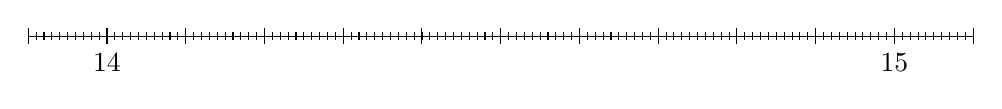
\begin{tikzpicture}
\draw (0,0) -- (12,0);
\foreach \x in {0,1,...,12} {\draw (\x,0.1cm) -- (\x,-0.1cm) ;}
\foreach \x in {0,0.1,...,12} {\draw (\x,0.05cm) -- (\x,-0.05cm);}
\draw (1,0.1cm) -- (1,-0.1cm) node[below] {$14$};
\draw (11,0.1cm) -- (11,-0.1cm) node[below] {$15$};
\ifdefined\isprof
	\draw[red] (6cm,0.25cm) -- (6cm,-0.25cm) node[above=0.4cm] {A\strut};
	\draw[red] (10.5cm,0.25cm) -- (10.5cm,-0.25cm) node[above=0.4cm] {B\strut};
	\draw[red] (10.3cm,0.25cm) -- (10.3cm,-0.25cm) node[above=0.4cm] {C\strut};
	\draw[red] (7.25cm,0.25cm) -- (7.25cm,-0.25cm) node[above=0.4cm] {D\strut};
\fi

\end{tikzpicture}

A(14,5) B(14,95) C(14,93) D(14,625)
\end{center}

\textbf{Exercice 5}: Range chaque liste dans l'ordre croissant
\begin{center}
12,4 - 1,24 - 12,04 - 1,204 - 12,42

\gap*{$1,204 < 1,24 < 12,04 < 12,4 < 12,42$}

0,98 - 0,908 - 0,098 - 0,89 - 0,809

\gap*{$0,098 < 0,809 < 0,89 < 0,908 < 0,98$}
\end{center}

\textbf{Exercice 6}: Encadre par deux entiers consécutifs les nombres suivants
\begin{center}
\begin{tabular}{ccc}

\gap*{1}$< 1,67 <$ \gap*{2} &\hspace{1cm}& \gap*{53} $< \phantom{00}53,8\phantom{0} <$ \gap*{54} \\ 

\gap*{0} $< 0,09 <$ \gap*{1} && \gap*{999} $< 999,67 <$ \gap*{1000} \\ 

\end{tabular} 
\end{center}


\end{document}